\documentclass[a4paper, platex, dvipdfmx]{jsarticle}
\usepackage{graphicx}
\usepackage{amsmath}
\begin{document}
方程式$f(x)=0$の解の近似値を求める方法を考えよう。
いくつかのアルゴリズムが知られているが、
ここでは二分法(第1章、p.1)およびニュートン法(第2章、p.2)を学習しよう。

ただし、ここでは次のことを仮定する。
\begin{itemize}
  \item $f$は区間$a\leq x\leq b$で単調増加であり、$f(a)<0$かつ$0<f(b)$を満たす。
\end{itemize}
これらの条件が満たされるとき、中間値の定理から、求める解$x$は$a\leq x\leq b$を満たす。
ここで考える関数$f$の例を、図1に示す。
\begin{figure}
  \centering
  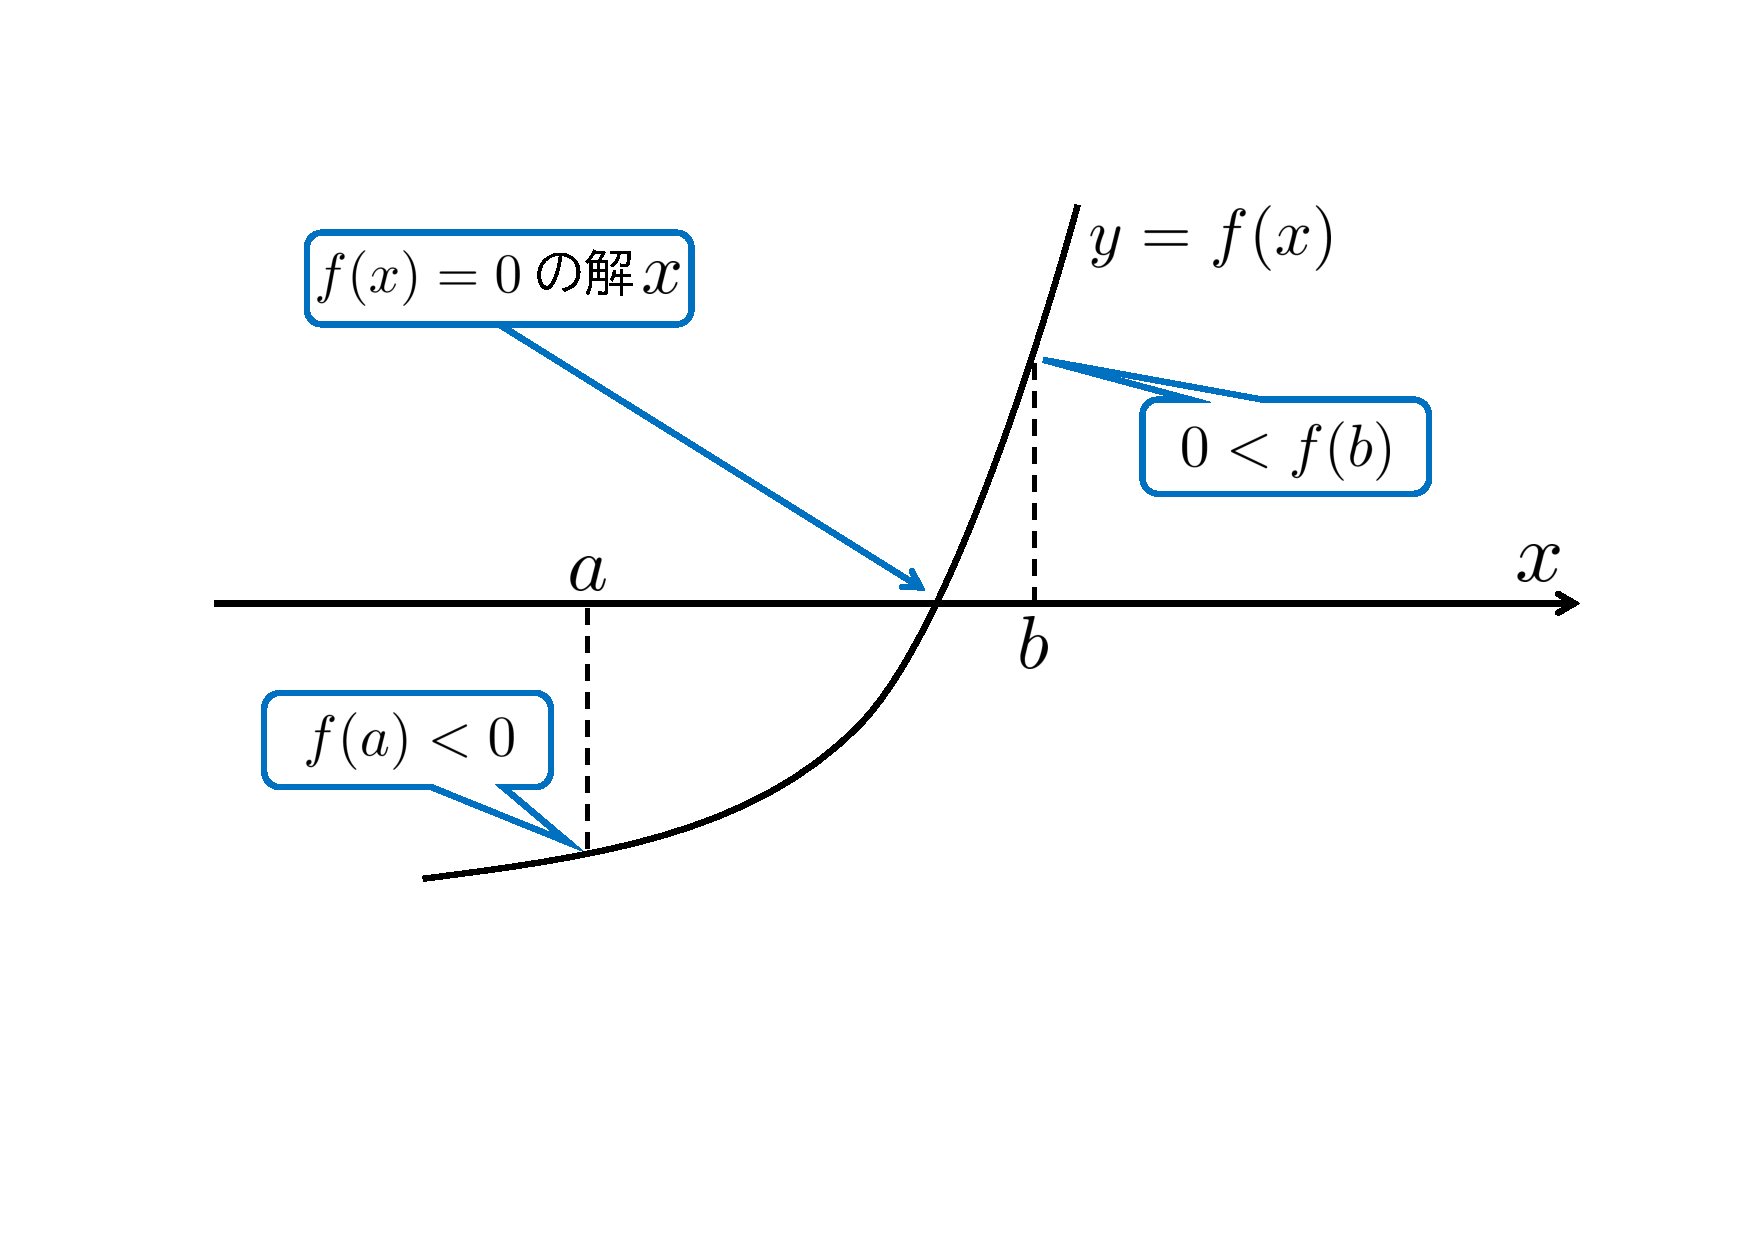
\includegraphics[width=10cm]{fig/figure1.pdf}
  \caption{ここで考える対象とする関数$f$の例。}
\end{figure}

\section{二分法}
\subsection{アルゴリズム}
二分法とは、次の手順を十分良い精度の解が得られるまで繰り返すアルゴリズムである。
\begin{enumerate}
  \item $c=(a+b)/2$を計算する。
  \item $0<f(c)$ならば、$b$を$c$で置き換える。$f(c)<0$ならば、$a$を$c$で置き換える。
\end{enumerate}
二分法のイメージ図を、図2に示す。図2では$0<f(c)$の場合を示している。
\begin{figure}
  \centering
  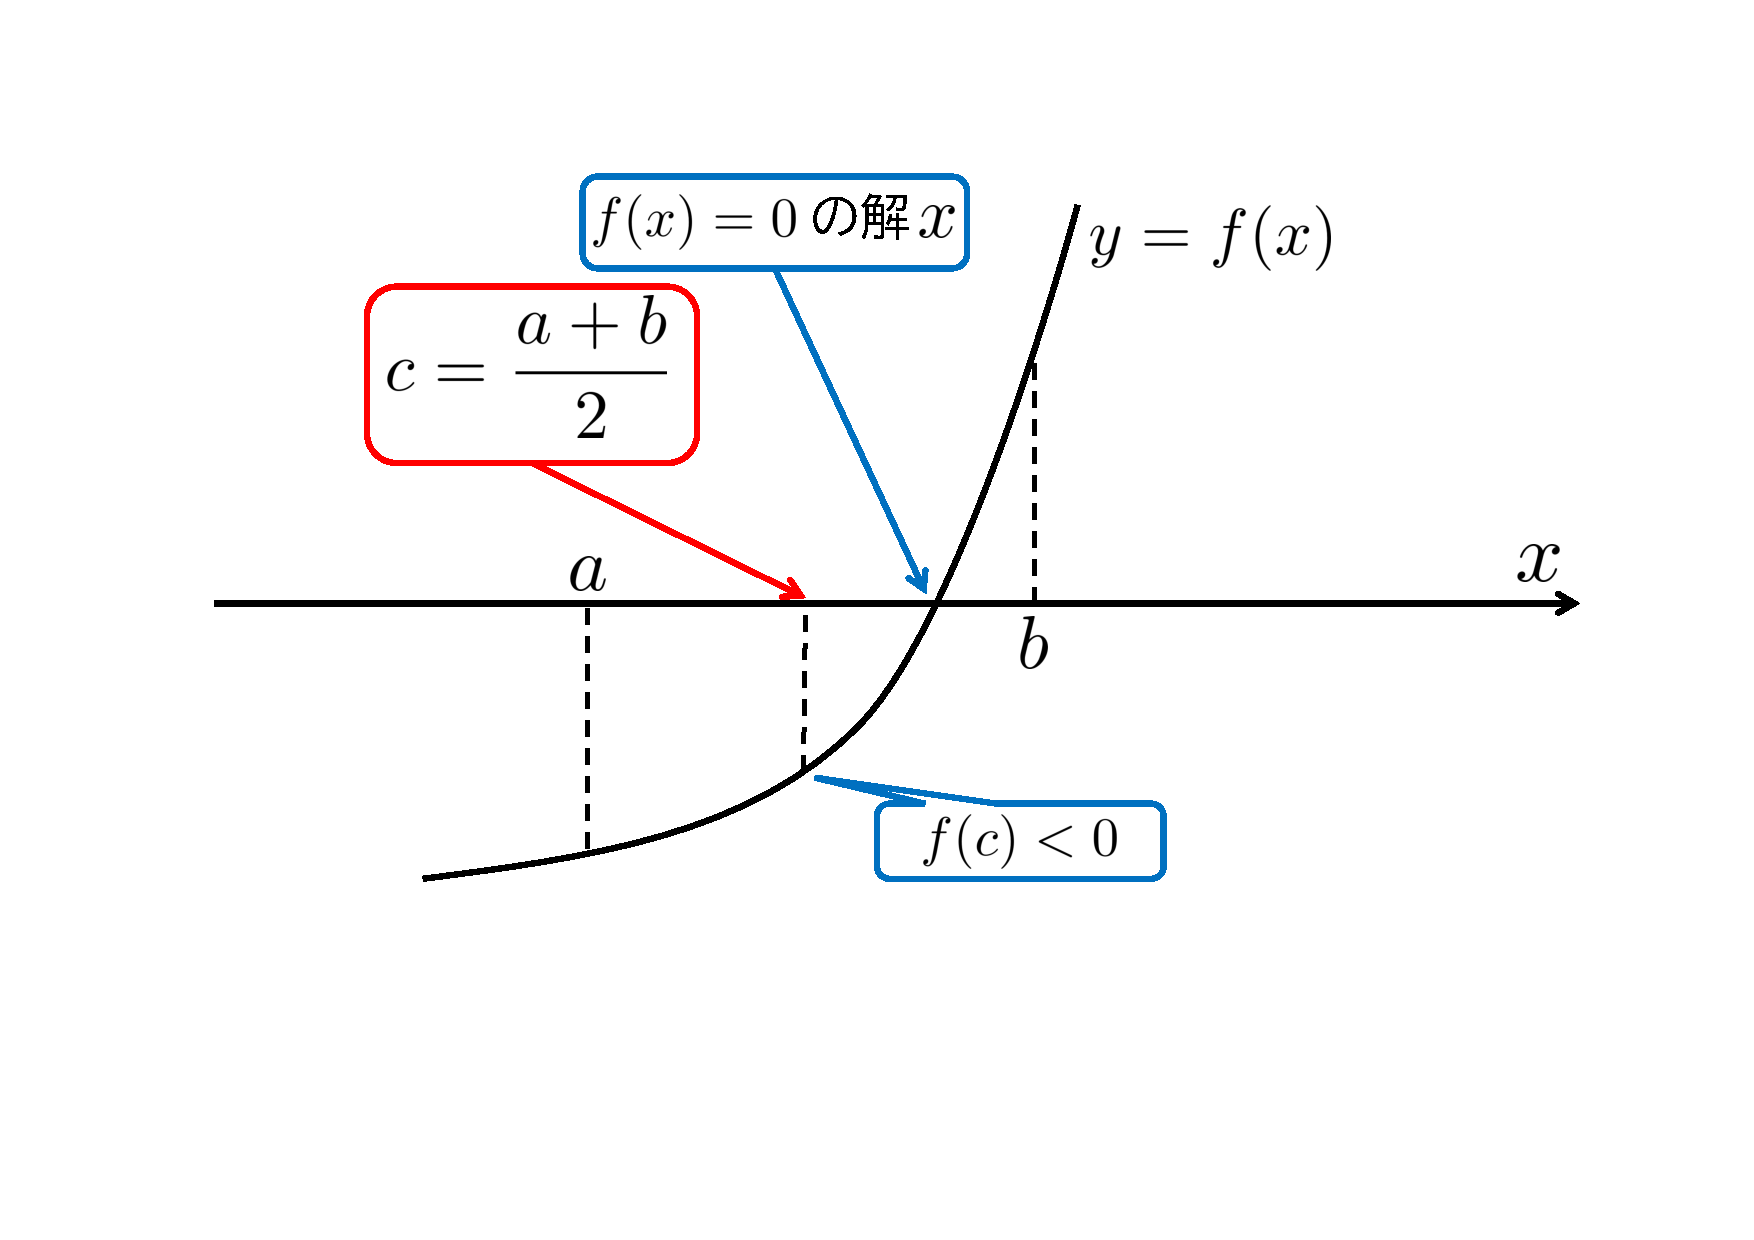
\includegraphics[width=10cm]{fig/figure2.pdf}
  \caption{二分法のイメージ図。}
\end{figure}
図から分かるように、$a\leq x\leq c$を満たす$x$は$f(x)=0$の解になり得ないので、
考えるべき区間は$c\leq x\leq b$に限られる。同じように考えることで、
解が存在しうる区間の幅を次々と半分にできる。
これを繰り返していけば、$a$と$b$はほぼ同じ値を取るようになるので、
このときの値を方程式$f(x)=0$の解の近似値とすればよい。

なお、二分法を一般化すると、有名な「二分探索」というアルゴリズムになる。
興味があれば、調べてみてほしい。

\subsection{例}
1.1節で説明したアルゴリズムの具体例を見てみよう。$f(x)=x^2-1$とすると、
$f(0)<0$かつ$0<f(3)$だから、方程式$f(x)=0$の解$x$は$0\leq x\leq 3$を満たす。
そこで、$(a,b)=(0,3)$としよう。
\begin{description}
  \item[1回目の繰り返し]
    $c=(a+b)/2=1.5$である。$0<f(c)$だから、$b$の値を$c$で置き換えて、$(a,b)=(0,1.5)$となる。
  \item[2回目の繰り返し]
    $c=(a+b)/2=0.75$である。$f(c)<0$だから、$a$の値を$c$で置き換えて、$(a,b)=(0.75,1)$となる。
  \item[3回目の繰り返し]
    $c=(a+b)/2=0.875$である。$f(c)<0$だから、$a$の値を$c$で置き換えて、$(a,b)=(0.875,1)$となる。
\end{description}
アルゴリズムの途中で$a$や$b$の値が変化することに注意しよう。2回目の繰り返しでは、1回目の繰り返しで
変化した$a,b$の値を用いる。

$a$と$b$の値は、方程式$f(x)=0$の解$x=1$に近づいていることがわかる。
何度も手順を繰り返せば、$a$と$b$の値はほぼ$1$になることが予想できるだろう。

\section{ニュートン法}
\subsection{アルゴリズム}
ニュートン法では、初期値$x_0=b$から、次のアルゴリズムに従って$x_1,x_2,\ldots$を
求めていく。
\begin{itemize}
  \item 点$x_n$における$y=f(x)$の接線と$x$軸の交点の$x$座標を、$x_{n+1}$とする。
\end{itemize}
このことを図で表すと、図3のようになる。
\begin{figure}
  \centering
  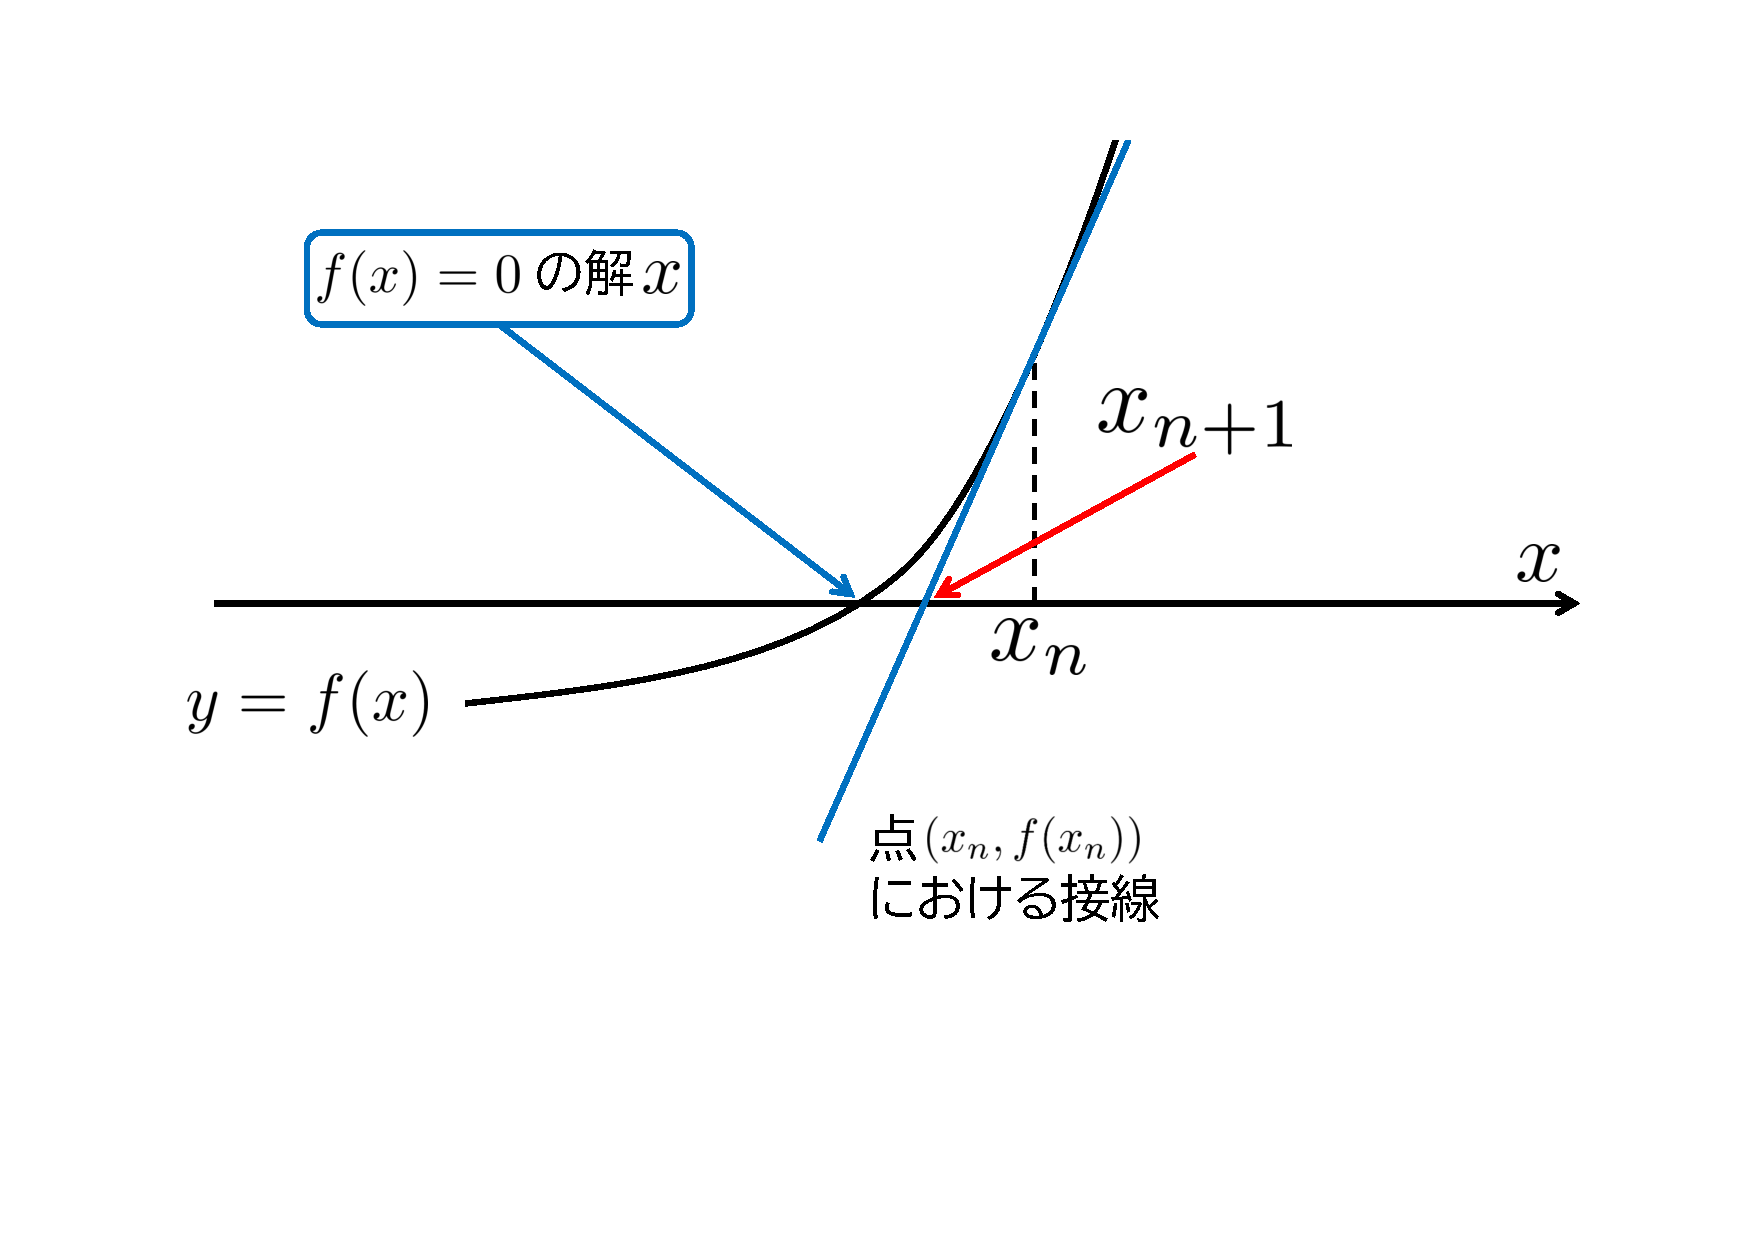
\includegraphics[width=10cm]{fig/figure3.pdf}
  \caption{ニュートン法のイメージ図。}
\end{figure}
また、式で書くと、次のようになる。なぜこの式になるのかは宿題とする。
\begin{align}
  x_{n+1}=x_n-\frac{f(x_n)}{f'(x_n)}
\end{align}
十分大きな整数$N$に対して、$x_N$を方程式の近似解とすればよい。
つまり、式(1)の操作を十分に繰り返せば、方程式$f(x)=0$の解の近似値が求められる。

ただし、$f'(x)$が存在し、かつこれが計算できないと、
ニュートン法は使えないことに注意する必要がある。

\subsection{例}
1.2節と同じ関数$f(x)$を例に、ニュートン法を実行してみよう。
$x_0=3$からスタートしてみよう。
$f'(x)=2x$だから、式(1)は次のように書き直せる。
\begin{align}
  x_{n+1}=x_n-\frac{{x_n}^2-1}{2x_n}=\frac{{x_n}^2+1}{2x_n}
\end{align}
式(2)の方が簡単なので、式(2)に従って計算してみよう。ただ計算するだけなので、結果だけを示す。
\begin{description}
  \item[1回目の繰り返し] $x_1=(3^2+1)/(2\cdot 3)=5/3=1.666\cdots$
  \item[2回目の繰り返し] $x_2=17/15=1.133\cdots$
  \item[3回目の繰り返し] $x_3=257/255=1.007\cdots$
\end{description}
このように、急速に解$x=1$に近づいていることがわかる。

\section{二分法とニュートン法の比較}
1.2節と2.2節から、ニュートン法の方が複雑である一方、より精度の良い値が
すぐに得られることが予想できる。そこで、もう少し複雑な関数
\begin{align}
  f(x)=-\cos\frac{x}{3}+\frac{1}{2}
\end{align}
で試してみよう。次のことがすぐにわかる(これらのことの確認は宿題とする)。
\begin{enumerate}
  \item $f(0)=-0.5,f(3\pi/2)=0.5$である。
  \item $f(x)$の導関数$f'(x)$は、
  \begin{align}
    f'(x)=\frac{1}{3}\sin\frac{x}{3}
  \end{align}
  である。
  \item $f(x)$は$0\leq x\leq 3\pi/2$で単調増加である
\end{enumerate}
したがって、二分法とニュートン法が両方利用できる。

二分法とニュートン法を両方適用したときの、方程式$f(x)=0$の解の近似値の推移を、
表1に示す。ただし、二分法は$(a+b)/2$の値を、ニュートン法は$x_n$の値を、
それぞれ示している。二分法は$(a,b)=(0,3\pi/2)$を、
ニュートン法は$x_0=3\pi/2$を、それぞれ初期値として与えた。
\begin{table}
  \centering
  \caption{二分法とニュートン法による$f(x)=0$の解の近似値の推移。小数第7位を四捨五入した。}
  \begin{tabular}{ccc}
    \hline
    繰り返し回数 & 二分法 & ニュートン法 \\\hline
    0 & 2.356194 & 4.712389 \\
    1 & 3.141976 & 3.212389 \\
    2 & 3.141401 & 3.142056 \\
    3 & 3.141689 & 3.141593 \\
    4 & 3.141545 & 3.141593 \\
    5 & 3.141617 & 3.141593 \\
    6 & 3.141581 & 3.141593 \\
    7 & 3.141599 & 3.141593 \\
    8 & 3.141590 & 3.141593 \\
    9 & 3.141594 & 3.141593 \\
    10 & 3.141592 & 3.141593 \\\hline
  \end{tabular}
\end{table}

ところで、方程式$f(x)=0$の解のうち$0\leq x\leq 3\pi/2$を満たすものは、
$x=\pi=3.1415926\cdots$である。このことと表1の
結果を見比べても、やはりニュートン法の方がより良い近似値を
何度も繰り返しアルゴリズムを実行することなく求められることがわかる。
\end{document}
